\chapter{Software Overview\label{sec:software}}

This chapter will serve as an overview of the functionality of the BLControl software. Figure~\ref{fig:ui} shows the full user interface that appears when the application is started. Each panel in the window is explained in its own section below.

\begin{figure}
\centering
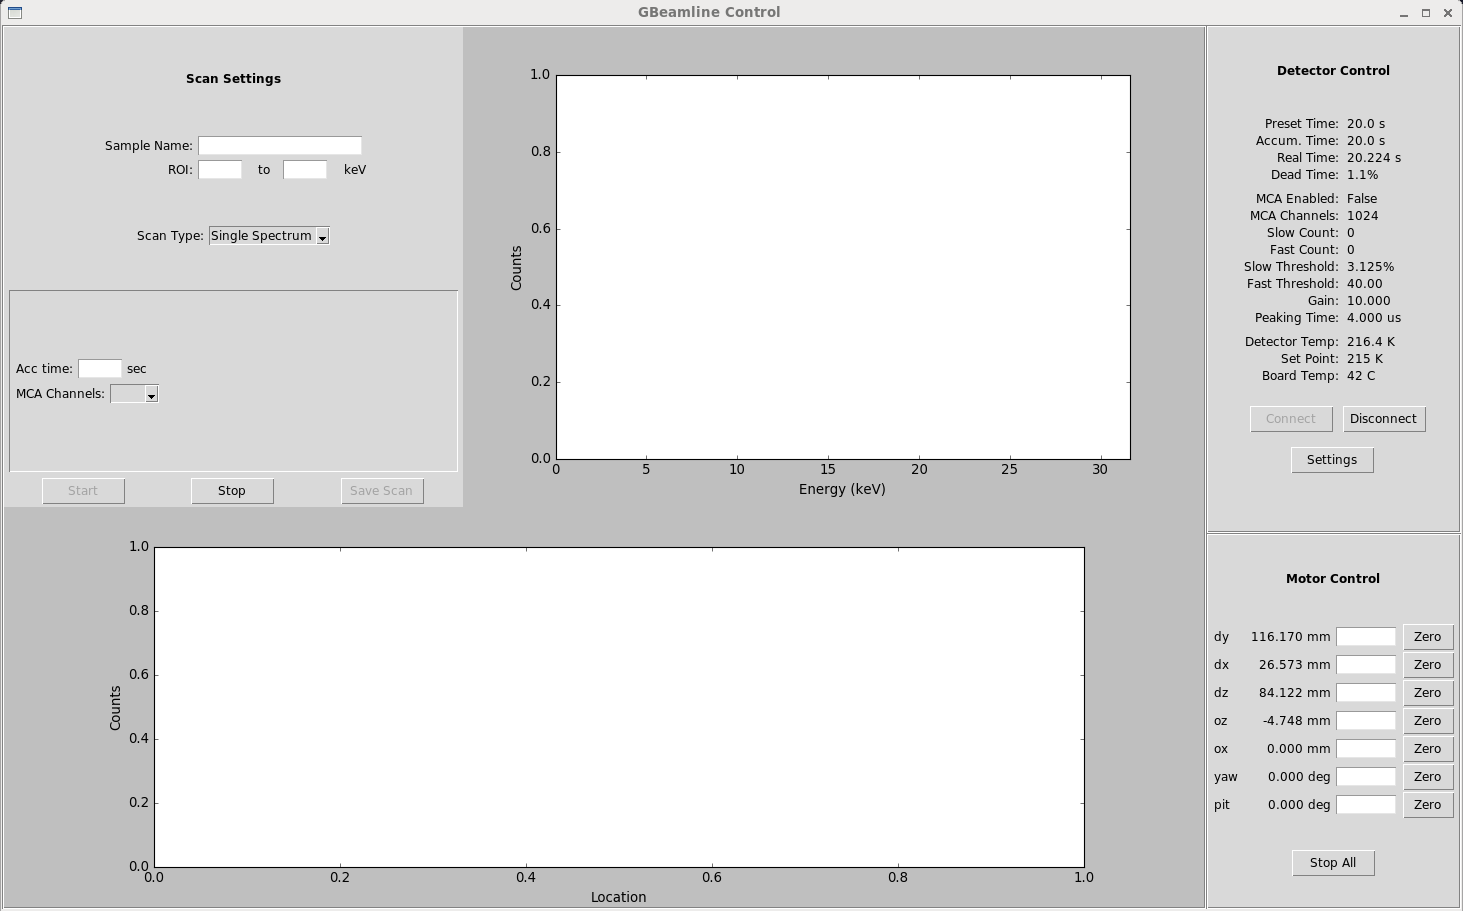
\includegraphics[width=0.7\textwidth]{fullui.png}
\caption{\label{fig:ui} Screenshot of the full user interface on startup. The elements of the interface, clockwise from top left, are the scan settings, the single spectrum plot, the detector status readout, the motor control panel, and the scan plot.}
\end{figure}

\section{Scan Settings}

\begin{figure}
\centering
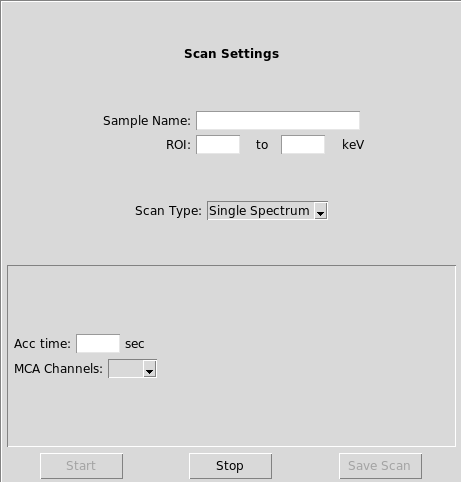
\includegraphics[width=0.5\textwidth]{scansettings.png}
\caption{\label{fig:scanset} The scan settings panel, with scan type set to ``Single Spectrum.''}
\end{figure}

The scan settings panel is shown in Fig.~\ref{fig:scanset}. The top half contains fields for setting a sample name and ROI (region of interest) and a drop-down menu for choosing a scan type.

The sample name field is only used to identify the sample in any saved files. You can put whatever you like here or leave it blank.

The ROI setting allows you to choose a region of the spectrum between two energy values to be analyzed in real-time along with the total spectrum. If this value is set, the ROI will be highlighted in the spectrum plot and information about the portion of the spectrum will be displayed on the plot. The counts in the ROI will also be counted separately in any scans that are run.

The dropdown menu allows you to choose what type of scan to run, with the choices being ``Single Spectrum,'' ``Linear Scan'' and ``Grid Scan.'' Each scan type is covered in more detail below. When the scan type is changed, the lower portion of the panel will change to display the settings available for that scan type.
For each scan type, press the ``Start'' button on the bottom of the scan settings panel to begin running the scan. The ``Stop'' button may be used to terminate the scan prematurely. Once a scan is finished or has been stopped by the user, the ``Save Scan'' button allows you to save the data from the most recent scan in a plaintext format.

\subsection{Single Spectrum}

Fig.~\ref{fig:scanset} shows the layout of the scan settings panel when ``Single Spectrum'' is selected. For a single spectrum, there are only two scan-specific options: the accumulation time, in seconds, and the number of MCA channels to be used. The accumulation time can be any value, and the number of channels is selectable from a drop down menu. The detector allows the use of 256, 512, 1024, 2048, 4096, or 8192 channels.

\begin{figure}
\centering
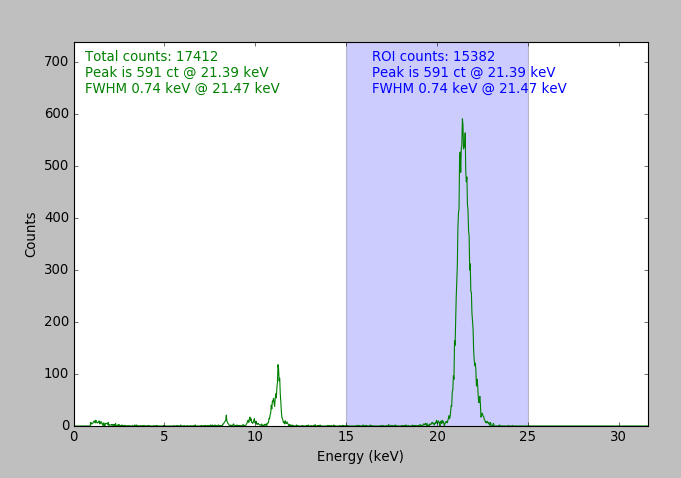
\includegraphics[width=0.7\textwidth]{specplot.png}
\caption{\label{fig:specplot} The spectrum plot display panel, during the collection of a single spectrum.}
\end{figure}

When the spectrum acquisition is started, after a few seconds the spectrum will begin to display in the spectrum plot display panel, to the right of the scan settings panel. This plot will update in real time (with the update frequency depending on the number of channels) until the acquisition is complete.

An example image of the spectrum plot is shown in Fig.~\ref{fig:specplot}. In the upper left corner, the green text displays some information about the spectrum: the total number of counts, the number of counts and the location of the peak channel, and the full width at half maximum (FWHM) and center of the highest peak in the spectrum.
For this spectrum, the ROI was set to 15-25 keV, and this region is highlighted in blue. The blue text in the upper right corner gives the similar information about the portion of the spectrum that is contained in the ROI. In this example, the highest peak in the ROI is the same as the highest peak in the full spectrum.

\subsection{Linear Scan}

A linear scan consists of moving a single stage over a distance in specified increments, and taking a spectrum at each position. This is useful during the alignment process, when you want to position each stage at the location that maximizes the count rate.

\begin{figure}
\centering
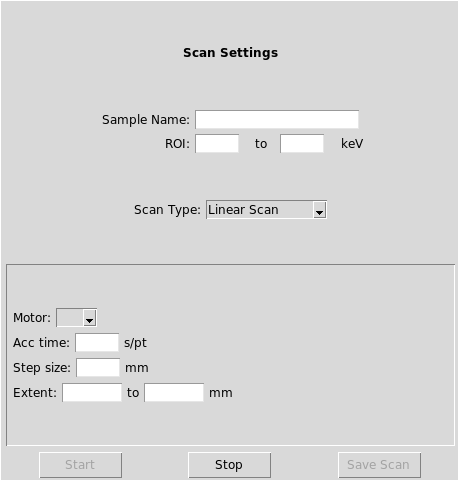
\includegraphics[width=0.5\textwidth]{linscan.png}
\caption{\label{fig:linscan} The scan settings panel when ``Linear Scan'' is selected.}
\end{figure}

Fig.~\ref{fig:linscan} shows the layout of the scan settings panel when ``Linear Scan'' is selected. A dropdown menu allows you to choose a motor to scan from the motors that are connected. The accumulation time field specifies the duration of the spectrum that will be taken at each position. Step size is the distance interval between each scan position. The default units are millimeters, but will change to degrees if a rotary stage is selected from the motor dropdown menu. Finally, the extent fields specify the beginning and ending points of the scan. The extent is inclusive, meaning a spectrum will be taken at the beginning of the interval, and, if the interval is exactly divisible by the step size, a spectrum will be taken at the end of the interval as well. Together, the extent and the step size define the number of points in a linear scan. The approximate duration of the scan can be determined from the accumulation time at each point and the number of points, but note that some extra time will be needed for data transfer and stage motion.

%spec display
While the scan is running, the spectra collected at each point will be displayed in the spectrum plot panel, similar to how it is displayed while collecting a single spectrum. During a scan, however, the number of MCA channels is limited to 256 to improve data transfer speed and decrease the size of the files generated from the scans. When the scan is finished, the stage will remain in the final location of the scan until moved by the user.

\begin{figure}
\centering
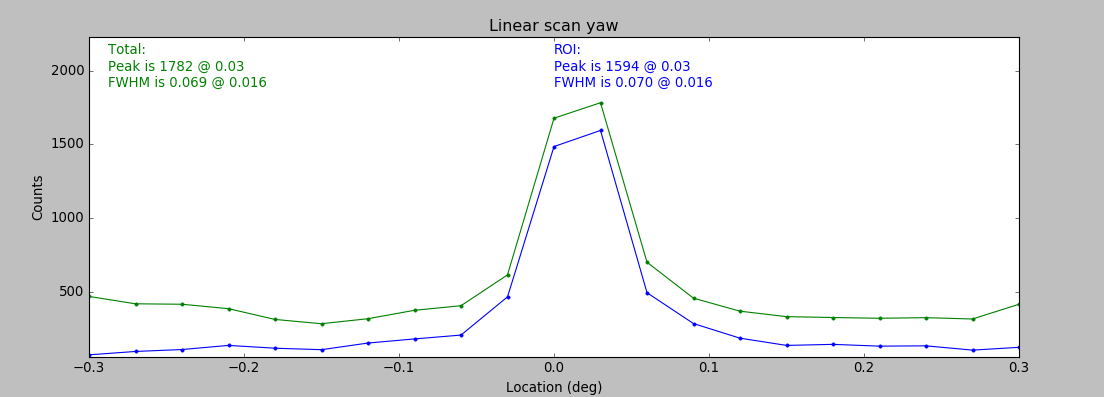
\includegraphics[width=\textwidth]{linplot.png}
\caption{\label{fig:linplot} The plot displayed in the scan plot display panel, after a linear scan is run.}
\end{figure}

%lin scan plot
A plot will also be generated in the scan plot panel, as shown in Fig.~\ref{fig:linplot}. In real time during the scan, the plot will show the total number of counts collected at each location in green, and the number of counts in the ROI (if used) in blue. Information is also displayed about the highest peak for both the total count data and the ROI data.

\subsection{Grid Scan}

A grid scan is a 2D scan of the detector in the $xy$ plane, which is useful for centering the detector on the axis of the optic. Fig.~\ref{fig:gridscan} displays the options for setting up a grid scan. The user specifies the accumulation time as in a linear scan. The step size is the distance between consecutive points in both the $x$ and $y$ directions. The grid size dropdown menu allows the user to specify the number of points to be collected, from $3 \times 3$ to $11 \times 11$ points (odd numbers only).

\begin{figure}
\centering
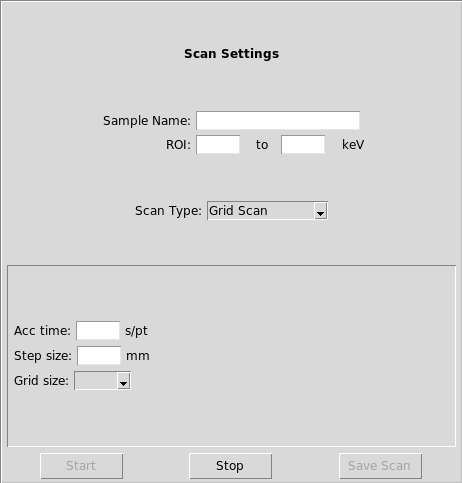
\includegraphics[width=0.5\textwidth]{gridscan.png}
\caption{\label{fig:gridscan} The scan settings panel when ``Grid Scan'' is selected.}
\end{figure}

Unlike the linear scan, which allows the user to specify the start and end points of a scan, a grid scan is always centered around the position of the detector at the time the scan is started. When the scan is initiated, the detector will move to the first position, the lowest values of $x$ and $y$, and proceed in a raster fashion until the scan is complete. First $x$ is scanned all the way across in units of the step size, then $y$ is incremented by one step and $x$ is scanned in the opposite direction, and so on until the entire area has been scanned. As in the linear scan, the spectra appear in the spectrum plot panel as they are acquired.

\begin{figure}
\centering
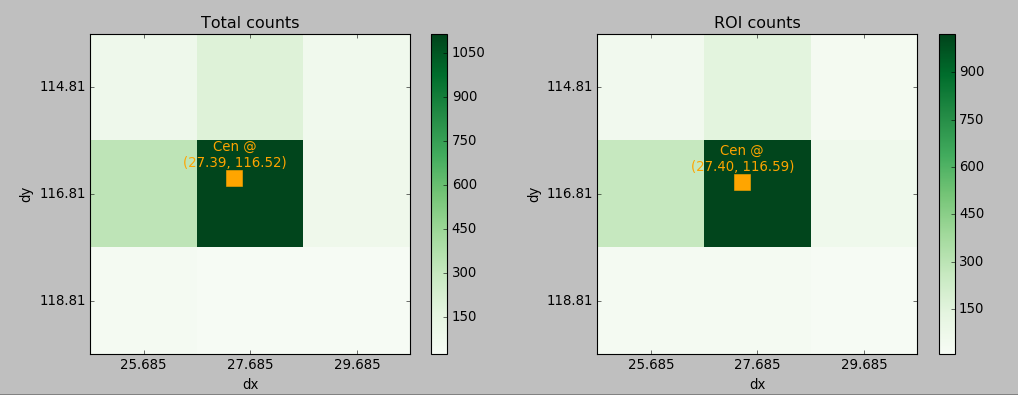
\includegraphics[width=\textwidth]{gridplot.png}
\caption{\label{fig:gridplot} The plot displayed in the scan plot display panel, after a grid scan is run.}
\end{figure}

The results of the scan are displayed in real time in the scan plot panel, shown in Fig.~\ref{fig:gridplot}. Points are filled in as they are collected, and points not yet collected appear in gray. The total counts are plotted on the left, and the counts in the ROI, if used, are plotted on the right.  Both plots display the calculated center of mass of the scans to aid the user in centering the detector. When the scan is finished, the detector will remain at the final point of the scan until moved by the user.

\section{Motor Control}

\begin{figure}
\centering
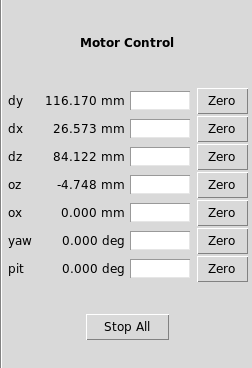
\includegraphics[width=0.35\textwidth]{motorctl.png}
\caption{\label{fig:motorctl} The motor control panel.}
\end{figure}

The user can move each stage independently using the motor control panel, shown in Fig.~\ref{fig:motorctl}. For each connected stage, the current position is shown, followed by a new position field and a ``Zero'' button. To move the stage to a new position, enter the new position in the field and press Enter. The current position will update in real time as the stage moves. You can also move the stages using the hardware knobs. The zero button will set the current position of the stage to zero. The ``Stop All'' button, located at the bottom of the panel, can be used for an emergency stop of all stages.

%homing
If the power has been disconnected to one of the stages since the last use, it must be homed before the next use, otherwise the encoder will not have a valid position reference. If one or more of the motors is unhomed when the software is started up, the user will be prevented from moving that motor. A warning message will appear, the new position field for the affected stages will be grayed out, and the ``Zero'' button will be replaced by a ``Home'' button. Pressing the ``Home'' button will instruct the stage controllers to perform the homing routine automatically, but \textbf{you must make sure the area is clear for the motor to return all the way to the home position} before performing this step. This includes ensuring that the stages will not run into any obstacles while homing, and that the cables connecting the motors will not become tangled or overstressed. Also, \textbf{the current position will be lost when the homing routine is performed}. For these reasons, it is often preferable to home the motors manually, by using the knob on the controller to move them until the home sensor is triggered. This allows you to move the motors slowly, make sure there are no obstacles in the way, and mark the current position of the stages before beginning the homing process.

%something about currents??

\section{Detector Control}

\begin{figure}
\centering
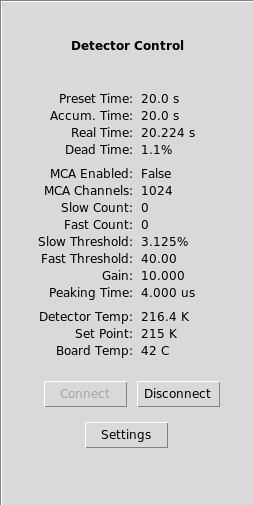
\includegraphics[width=0.35\textwidth]{detctl.png}
\caption{\label{fig:detctl} The detector status panel.}
\end{figure}

\begin{figure}
\centering
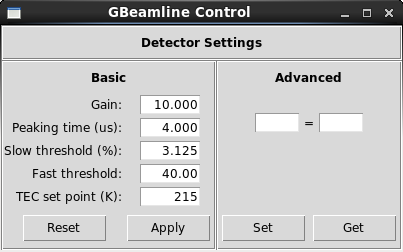
\includegraphics[width=0.5\textwidth]{detsettings.png}
\caption{\label{fig:detsettings} The detector settings popup window.}
\end{figure}

\section{Configuration Files}
